\documentclass{paper}

%\usepackage{times}
\usepackage{epsfig}
\usepackage{graphicx}
\usepackage{amsmath}
\usepackage{amssymb}
\usepackage{color}
\usepackage{caption}
\usepackage{subcaption}

% load package with ``framed'' and ``numbered'' option.
%\usepackage[framed,numbered,autolinebreaks,useliterate]{mcode}

% something NOT relevant to the usage of the package.
\setlength{\parindent}{0pt}
\setlength{\parskip}{18pt}






\usepackage[latin1]{inputenc} 
\usepackage[T1]{fontenc} 

\usepackage{listings} 

\newcommand{\equationinalign}[1]{%
  \multispan{2}%
  \hfill$\displaystyle{#1}$\hfill
  \ignorespaces
}

\lstset{% 
   language=Python, 
   basicstyle=\small\ttfamily, 
} 



\title{Assignment 1}



\author{Nalet Meinen\\13-463-955}
% //////////////////////////////////////////////////


\begin{document}



\maketitle


% Add figures:
%\begin{figure}[t]
%%\begin{center}
%\quad\quad   \includegraphics[width=1\linewidth]{ass2}
%%\end{center}
%
%\label{fig:performance}
%\end{figure}

\section*{Image blending}

\begin{enumerate}
\item \textbf{Exercise 1}

We can use a forward approach as it much simple to implement and it is sufficient for our needs. This derivation was discussed in the lecture.

\begin{align*}
   \lVert \Delta u \rVert_2 \simeq \sum_{i,j} \sqrt{ u[i+1,j] - u[i,j]^2 + ( u[i,j + 1] - u[i,j] )^2 }
\end{align*}

\item \textbf{Exercise 2}

\begin{figure}[!htb]
   \centering
   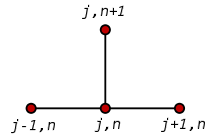
\includegraphics[width=0.3\textwidth]{images/stencil.png}
   \caption{Standard stencil as template}
 \end{figure}

\begin{align*}
   |u_C-g_C|^2_\Omega &= \sum_{i,j} \Omega[i,j] | u_C[i,j] - g_C[i,j] |^2_2 \\
   \frac{\partial}{\partial u[p,q]} |u_C-g_C|^2_\Omega &= \frac{\partial}{\partial u[p,q]} \sum_{i,j} \Omega[i,j] | u_C[i,j] - g_C[i,j] |^2_2
\end{align*}
\begin{align*}
   \frac{\partial}{\partial u[p,q]} \sum_{i,j} \Omega[i,j] | u_C[i,j] - g_C[i,j] |^2_2 &= 2 \cdot \Omega[i,j] \cdot ( u_C[i,j] - g_C[i,j] ) \\
   \frac{\partial |u_C-g_C|^2_\Omega}{\partial u[i,j]} &= \Omega[i,j] \cdot ( 2 \cdot u_C[i,j] - u_C[i+1,j] - u_C[i,j+1] \\
   & \quad \; - 2 \cdot g_C[i,j] + g_C[i-1,j] + g_C[i,j-1] )^2
\end{align*}

\pagebreak
\item \textbf{Implementation.} For each of the 3 solvers (gradient descent, \\ 
                               Linearization+Gauss-Seidel, Linearization+SOR):

For GD the results are quite good. However, for LGS and LSOR the numbers of iterations are a fixed value. A better result is achivable with a while loop in GD. In this case the running time for this notebook is already 40 minutes.

\textit{\textbf{Hint:} The numbers over the gradient images are the iterations for a image.}

\begin{itemize}
\item \textbf{Gradient Descent}
   \begin{figure}[!htb]
      \begin{tabular}[b]{cc}
      \begin{tabular}[b]{c}
         \begin{subfigure}[b]{0.4\columnwidth}
            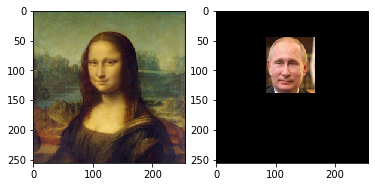
\includegraphics[width=\textwidth]{images/GD_input.png}
            \caption{GD input}
         \end{subfigure}\\
         \begin{subfigure}[b]{0.4\columnwidth}
            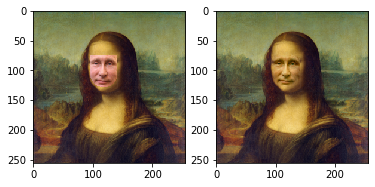
\includegraphics[width=\textwidth]{images/GD_output.png}
            \caption{GD output}
         \end{subfigure}
      \end{tabular}
      &
      \begin{tabular}[b]{c}
         \begin{subfigure}[b]{0.4\columnwidth}
            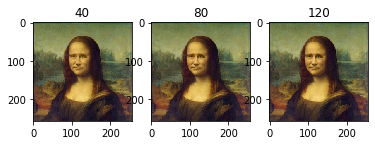
\includegraphics[width=\textwidth]{images/GD_gradient.png}
            \caption{GD gradient}
         \end{subfigure}\\
         \begin{subfigure}[b]{0.4\columnwidth}
            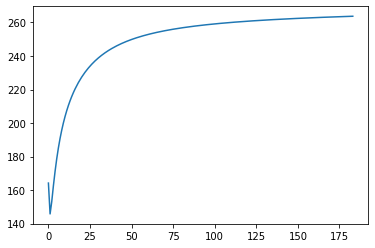
\includegraphics[width=\textwidth]{images/GD_energy.png}
            \caption{GD energy \\ (y: Energy, x: Iterations)}
         \end{subfigure}
      \end{tabular}
      \end{tabular}
      \caption{Result Gradient Descent}
   \end{figure}

\item \textbf{Linearization+Gauss-Seidel}
   \begin{figure}[!htb]
      \begin{tabular}[b]{cc}
      \begin{tabular}[b]{c}
         \begin{subfigure}[b]{0.4\columnwidth}
            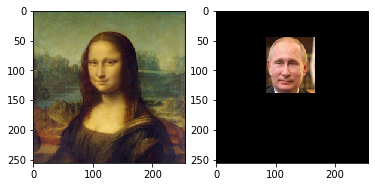
\includegraphics[width=\textwidth]{images/LGS_input.png}
            \caption{LGS input}
         \end{subfigure}\\
         \begin{subfigure}[b]{0.4\columnwidth}
            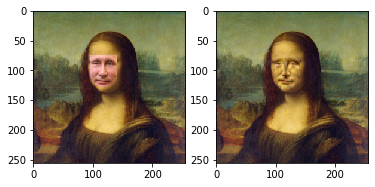
\includegraphics[width=\textwidth]{images/LGS_output.png}
            \caption{LGS output}
         \end{subfigure}
      \end{tabular}
      &
      \begin{tabular}[b]{c}
         \begin{subfigure}[b]{0.4\columnwidth}
            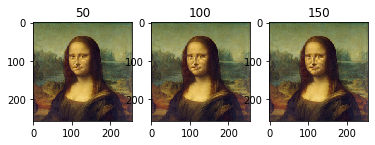
\includegraphics[width=\textwidth]{images/LGS_gradient.png}
            \caption{LGS gradient}
         \end{subfigure}\\
         \begin{subfigure}[b]{0.4\columnwidth}
            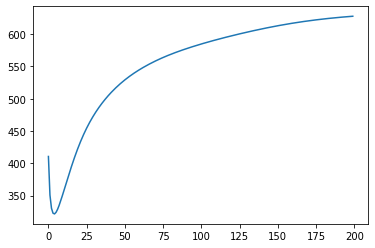
\includegraphics[width=\textwidth]{images/LGS_energy.png}
            \caption{LGS energy \\ (y: Energy, x: Iterations)}
         \end{subfigure}
      \end{tabular}
      \end{tabular}
      \caption{Result Gradient Descent}
   \end{figure}
\pagebreak
\item \textbf{Linearization+SOR}
\begin{figure}[!htb]
   \begin{tabular}[b]{cc}
   \begin{tabular}[b]{c}
      \begin{subfigure}[b]{0.4\columnwidth}
         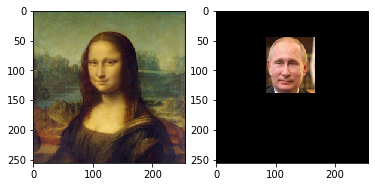
\includegraphics[width=\textwidth]{images/LSOR_input.png}
         \caption{LSOR input}
      \end{subfigure}\\
      \begin{subfigure}[b]{0.4\columnwidth}
         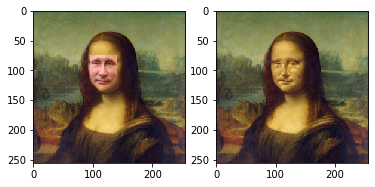
\includegraphics[width=\textwidth]{images/LSOR_output.png}
         \caption{LSOR output}
      \end{subfigure}
   \end{tabular}
   &
   \begin{tabular}[b]{c}
      \begin{subfigure}[b]{0.4\columnwidth}
         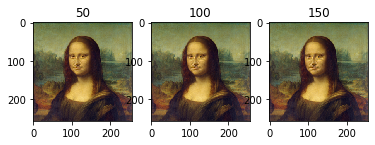
\includegraphics[width=\textwidth]{images/LSOR_gradient.png}
         \caption{LSOR gradient}
      \end{subfigure}\\
      \begin{subfigure}[b]{0.4\columnwidth}
         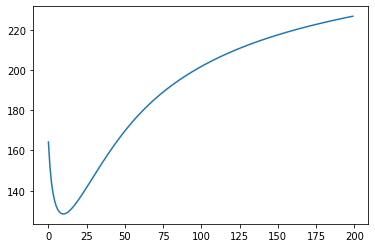
\includegraphics[width=\textwidth]{images/LSOR_energy.png}
         \caption{LSOR energy \\ (y: Energy, x: Iterations)}
      \end{subfigure}
   \end{tabular}
   \end{tabular}
   \caption{Result Gradient Descent}
\end{figure}
\end{itemize}

\pagebreak
\item \textbf{State which of the 3 solvers you choose. Show images obtained by very high, very low and manually-tuned (approximately optimal) $\lambda$.} In this section you should:

Very high lamda GD: 20, LGS: 50, LSOR: 20

\begin{itemize}
   \item \textbf{Gradient Descent}
      \begin{figure}[!htb]
         \begin{tabular}[b]{cc}
         \begin{tabular}[b]{c}
            \begin{subfigure}[b]{0.4\columnwidth}
               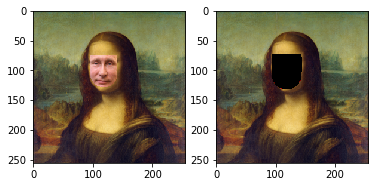
\includegraphics[width=\textwidth]{images/LH_GD_output.png}
               \caption{GD input}
            \end{subfigure}\\
            \begin{subfigure}[b]{0.4\columnwidth}
               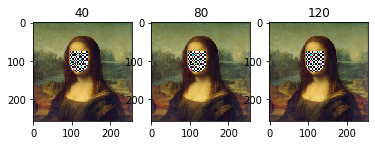
\includegraphics[width=\textwidth]{images/LH_GD_gradient.png}
               \caption{GD output}
            \end{subfigure}
         \end{tabular}
         &
         \begin{tabular}[b]{c}
            \begin{subfigure}[b]{0.4\columnwidth}
               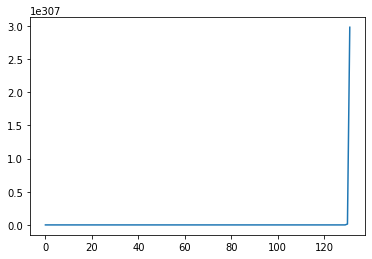
\includegraphics[width=\textwidth]{images/LH_GD_energy.png}
               \caption{GD energy \\ (y: Energy, x: Iterations)}
            \end{subfigure}
         \end{tabular}
         \end{tabular}
         \caption{Result Gradient Descent}
      \end{figure}
   
   \item \textbf{Linearization+Gauss-Seidel}
   \begin{figure}[!htb]
      \begin{tabular}[b]{cc}
      \begin{tabular}[b]{c}
         \begin{subfigure}[b]{0.4\columnwidth}
            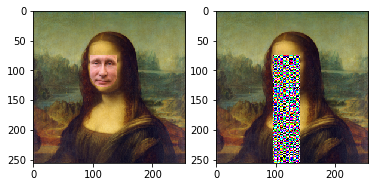
\includegraphics[width=\textwidth]{images/LH_LGS_output.png}
            \caption{LGS input}
         \end{subfigure}\\
         \begin{subfigure}[b]{0.4\columnwidth}
            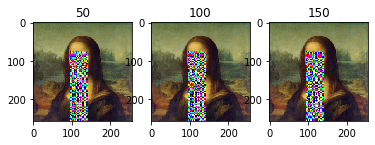
\includegraphics[width=\textwidth]{images/LH_LGS_gradient.png}
            \caption{LGS output}
         \end{subfigure}
      \end{tabular}
      &
      \begin{tabular}[b]{c}
         \begin{subfigure}[b]{0.4\columnwidth}
            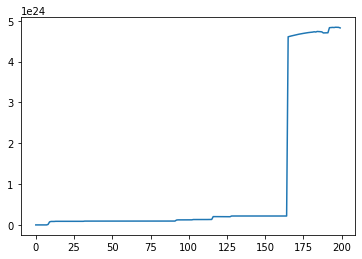
\includegraphics[width=\textwidth]{images/LH_LGS_energy.png}
            \caption{LGS energy \\ (y: Energy, x: Iterations)}
         \end{subfigure}
      \end{tabular}
      \end{tabular}
      \caption{Result Gradient Descent}
   \end{figure}

   \pagebreak
   \item \textbf{Linearization+SOR}
   \begin{figure}[!htb]
      \begin{tabular}[b]{cc}
      \begin{tabular}[b]{c}
         \begin{subfigure}[b]{0.4\columnwidth}
            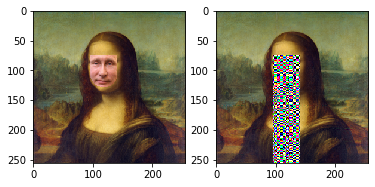
\includegraphics[width=\textwidth]{images/LH_LSOR_output.png}
            \caption{LSOR input}
         \end{subfigure}\\
         \begin{subfigure}[b]{0.4\columnwidth}
            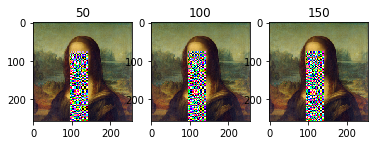
\includegraphics[width=\textwidth]{images/LH_LSOR_gradient.png}
            \caption{LSOR output}
         \end{subfigure}
      \end{tabular}
      &
      \begin{tabular}[b]{c}
         \begin{subfigure}[b]{0.4\columnwidth}
            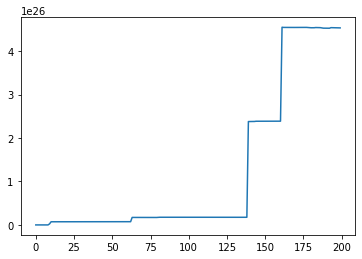
\includegraphics[width=\textwidth]{images/LH_LSOR_energy.png}
            \caption{LSOR energy \\ (y: Energy, x: Iterations)}
         \end{subfigure}
      \end{tabular}
      \end{tabular}
      \caption{Result Gradient Descent}
   \end{figure}
   \end{itemize}

Very low lamda GD: 2/100, LGS: 5/100, LSOR: 2/100

\begin{itemize}
\item \textbf{Gradient Descent}
   \begin{figure}[!htb]
      \begin{tabular}[b]{cc}
      \begin{tabular}[b]{c}
         \begin{subfigure}[b]{0.4\columnwidth}
            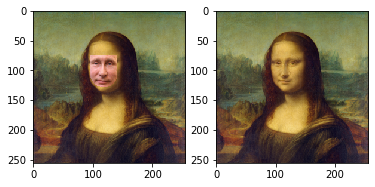
\includegraphics[width=\textwidth]{images/LL_GD_output.png}
            \caption{GD input}
         \end{subfigure}\\
         \begin{subfigure}[b]{0.4\columnwidth}
            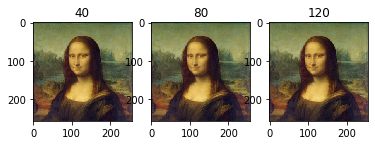
\includegraphics[width=\textwidth]{images/LL_GD_gradient.png}
            \caption{GD output}
         \end{subfigure}
      \end{tabular}
      &
      \begin{tabular}[b]{c}
         \begin{subfigure}[b]{0.4\columnwidth}
            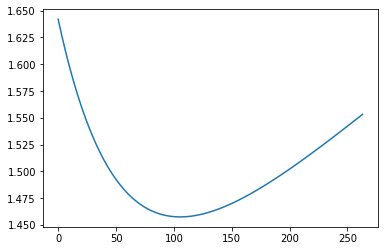
\includegraphics[width=\textwidth]{images/LL_GD_energy.png}
            \caption{GD energy \\ (y: Energy, x: Iterations)}
         \end{subfigure}
      \end{tabular}
      \end{tabular}
      \caption{Result Gradient Descent}
   \end{figure}
\pagebreak
\item \textbf{Linearization+Gauss-Seidel}
\begin{figure}[!htb]
   \begin{tabular}[b]{cc}
   \begin{tabular}[b]{c}
      \begin{subfigure}[b]{0.4\columnwidth}
         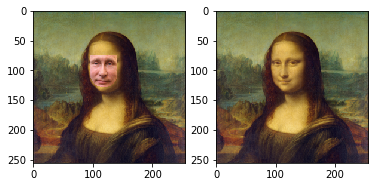
\includegraphics[width=\textwidth]{images/LL_LGS_output.png}
         \caption{LGS input}
      \end{subfigure}\\
      \begin{subfigure}[b]{0.4\columnwidth}
         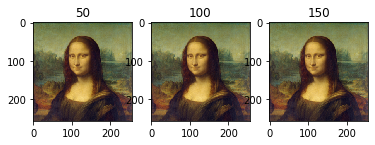
\includegraphics[width=\textwidth]{images/LL_LGS_gradient.png}
         \caption{LGS output}
      \end{subfigure}
   \end{tabular}
   &
   \begin{tabular}[b]{c}
      \begin{subfigure}[b]{0.4\columnwidth}
         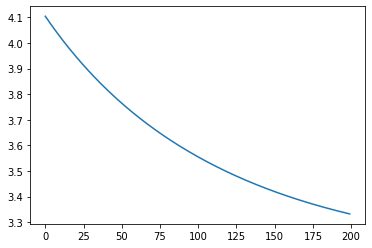
\includegraphics[width=\textwidth]{images/LL_LGS_energy.png}
         \caption{LGS energy \\ (y: Energy, x: Iterations)}
      \end{subfigure}
   \end{tabular}
   \end{tabular}
   \caption{Result Gradient Descent}
\end{figure}

\item \textbf{Linearization+SOR}
\begin{figure}[!htb]
   \begin{tabular}[b]{cc}
   \begin{tabular}[b]{c}
      \begin{subfigure}[b]{0.4\columnwidth}
         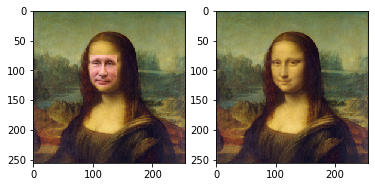
\includegraphics[width=\textwidth]{images/LL_LSOR_output.png}
         \caption{LSOR input}
      \end{subfigure}\\
      \begin{subfigure}[b]{0.4\columnwidth}
         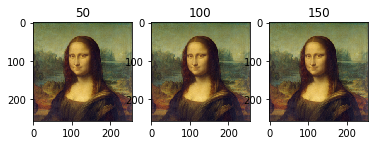
\includegraphics[width=\textwidth]{images/LL_LSOR_gradient.png}
         \caption{LSOR output}
      \end{subfigure}
   \end{tabular}
   &
   \begin{tabular}[b]{c}
      \begin{subfigure}[b]{0.4\columnwidth}
         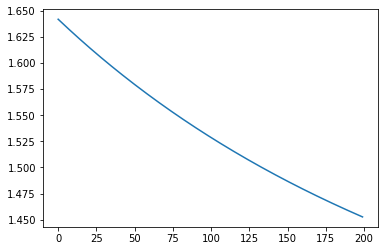
\includegraphics[width=\textwidth]{images/LL_LSOR_energy.png}
         \caption{LSOR energy \\ (y: Energy, x: Iterations)}
      \end{subfigure}
   \end{tabular}
   \end{tabular}
   \caption{Result Gradient Descent}
\end{figure}
\end{itemize}

\begin{itemize}
\item Describe the effect of $\lambda$ on the solution. \\
      $\lambda$ describes the change made to an image in each iteration step. Large $\lambda$ will lead to a large step size, which the solver cannot process. Small $\lambda$ would show no change at all at the images, as seen in the examples above.

\end{itemize}

\pagebreak
\item \textbf{Image blending:} 
\begin{itemize}
\item Display your own image composition here along with the foreground, background and mask images.
\item \textbf{Gradient Descent}
   \begin{figure}[!htb]
      \begin{tabular}[b]{cc}
      \begin{tabular}[b]{c}
         \begin{subfigure}[b]{0.4\columnwidth}
            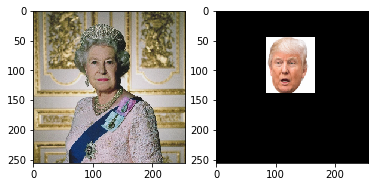
\includegraphics[width=\textwidth]{images/GD_trump_input.png}
            \caption{GD input}
         \end{subfigure}\\
         \begin{subfigure}[b]{0.4\columnwidth}
            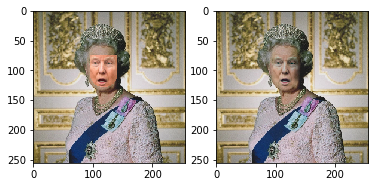
\includegraphics[width=\textwidth]{images/GD_trump_output.png}
            \caption{GD output}
         \end{subfigure}
      \end{tabular}
      &
      \begin{tabular}[b]{c}
         \begin{subfigure}[b]{0.4\columnwidth}
            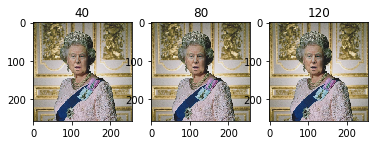
\includegraphics[width=\textwidth]{images/GD_trump_gradient.png}
            \caption{GD gradient}
         \end{subfigure}\\
         \begin{subfigure}[b]{0.4\columnwidth}
            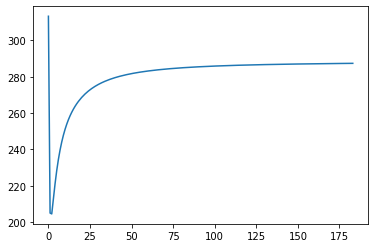
\includegraphics[width=\textwidth]{images/GD_trump_energy.png}
            \caption{GD energy \\ (y: Energy, x: Iterations)}
         \end{subfigure}
      \end{tabular}
      \end{tabular}
      \caption{Result Gradient Descent}
   \end{figure}
\item Describe how you used or modified the code to create your image(s).\\
      In this case the same images specs where used, so only the loading of the images needed to change.
\end{itemize}


\end{enumerate}


 \end{document}
 
 